% supplementary file for Accurate and Efficient Network-based Gene Function Prediction for Pathogenic Bacteria
%\documentclass{article}

%% Sets page size and margins
%\usepackage[margin=0.7in]{geometry}


\renewcommand{\thefigure}{S\arabic{figure}}
\renewcommand{\thetable}{S\arabic{table}}

\setcounter{figure}{0}
\clearpage
\appendix

% not sure how to make this an actual supplementary file
% appendix works for now 
%\title{Supplementary for Accurate and Efficient Network-based Gene Function Prediction for Pathogenic~Bacteria}
%\author[1]{Jeffrey N. Law}
%\author[2]{Shiv D. Kale}
%\author[3]{T. M. Murali}
%\affil[1]{Genetics, Bioinformatics, and Computational Biology Ph.D. program, Virginia~Tech, Blacksburg VA}
%\affil[2]{Biocomplexity Institute, Virginia Tech, Blacksburg VA}
%\affil[3]{Department of Computer Science, Virginia Tech, Blacksburg VA}
%%\affil[4]{ICTAS Center for Systems Biology of Engineered Tissues, Virginia Tech, Blacksburg VA}
%\date{September 2018}
%
%\maketitle

\section{Network Sizes}

Table \ref{tab:net-sizes} shows the number of nodes and edges for various BLAST \eval and STRING cutoffs.

\begin{table}[htb]
    \centering
\begin{tabular}{ccrr}
\SSN \eval & STRING &  & \\
cutoff & cutoff & \# Nodes & \# Edges \\
\hline
\e{-25} & - & 62,226 & 701,966\\
\e{-25} & 400 & 71,947 & 1,877,431\\
\e{-15} & - & 65,825 & 1,121,470\\
\e{-6} & - & 69,386 & 1,699,808\\
0.1 & - & 72,578 & 2,452,339\\
0.1 & 700 & 74,857 & 2,776,002\\
0.1 & 400 & 75,895 & 3,607,442\\
0.1 & 150 & 75,901 & 7,857,418\\
5 & - & 78,200 & 2,913,320\\
20 & - & 79,783 & 3,694,193\\
50 & - & 79,826 & 5,116,441\\
\end{tabular}
    \caption{Network sizes for various BLAST \eval and STRING cutoffs. }
    \label{tab:net-sizes}
\end{table}


\section{\birgrank results}
\label{sec:loso-birgrank}
\birgrank unfortunately did not perform as well as the other methods in our \loso evaluations. 
In the original evaluations of Jiang \textit{et al.}, they performed an evaluation where they whithheld all annotations from a given percentage of proteins and compared the ability of different algorithms to recover them. 
They observed that in this evaluation, their methods (\birgrank and AptRank) were not able to do better than \genemania and other methods. 
Our \loso evaluation seems to have exacerbated the problem for \birgrank. 
We varied the $\alpha$, $\theta$ and $\lambda$ parameters, but did not observe any improvement (results not shown).
\jeff{For five-fold cross-validation, \birgrank performed much better than \sinksource and \genemania (resuls not shown)}.

\section{MF Results}

\begin{figure}[H]
    \centering
    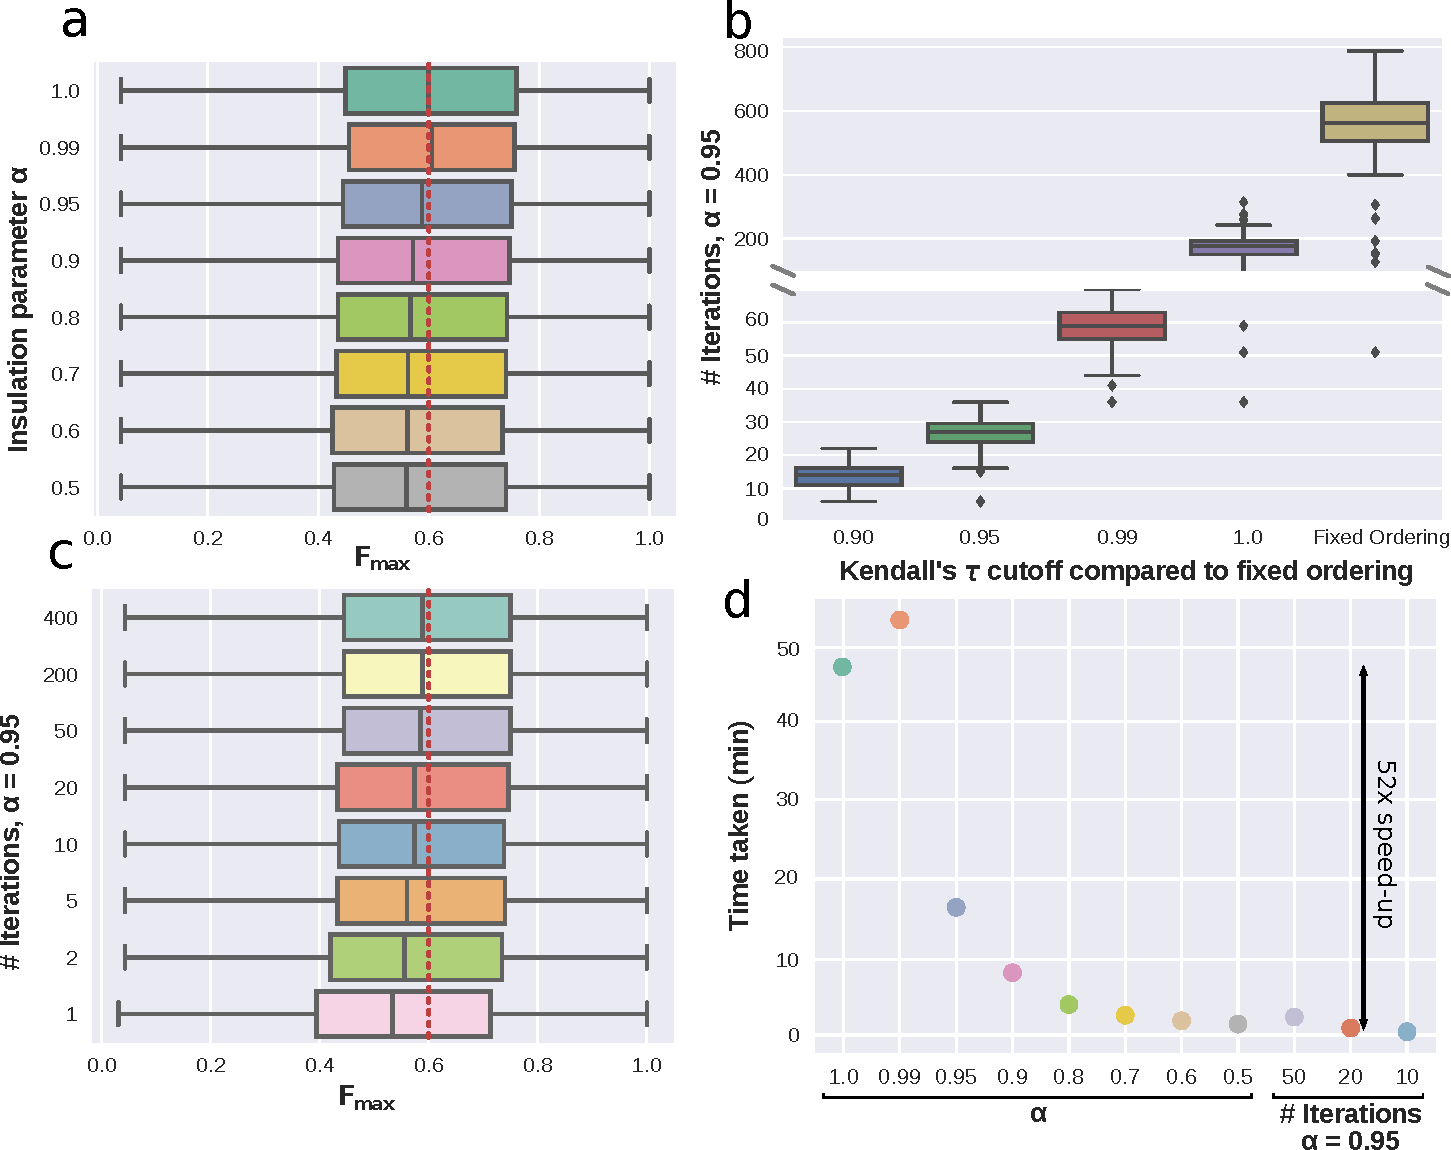
\includegraphics[width=\textwidth]{supp-figs/fig1-2018_06-seq-sim-e0_1-expc-rem-neg-comp-iea-50-1000-mf-a0_95.pdf}
    \caption{Trade-off between accuracy and speed for \sinksource on the 19 bacterial species \SSN (\eval <= 0.1) with 117 MF GO terms ($\ge 50$ annotations) for the \loso evaluation. 
      %Performance is measured by computing the \fmax on a GO term by GO term basis. Here we used annotations of BP GO terms with experimental evidence codes
      (\textbf{a}) Variation of \fmax distributions with $\alpha$. The vertical red dotted line represents the median \fmax for $\alpha = 1.0$.
      (\textbf{b}) Number of iterations required to fix the rankings of the left-out positives and negatives, or to reach a specified value of \ktau in comparison to the fixed ranking.
      (\textbf{c}) Variation of \fmax distributions with the number of iterations ($\alpha=0.95$). The vertical red dotted line represents the median \fmax for $\alpha = 1.0$ in panel (a).
      (\textbf{d}) Total time taken by \sinksource (shown in a and b) while varying $\alpha$ or the number of iterations with $\alpha=0.95$. Colors are the same as in (\textbf{a}) and (\textbf{c}).
    }
    \label{fig:sinksource-speed-vs-accuracy-mf}
\end{figure}


%\jeff{MF SinkSource increase from e1e-25 to e0_1 rank-sum test \pval $2.6\times{}10^{-7}$ )}
\begin{figure}[H]
    \centering
    %\jeff{figure placeholder}
    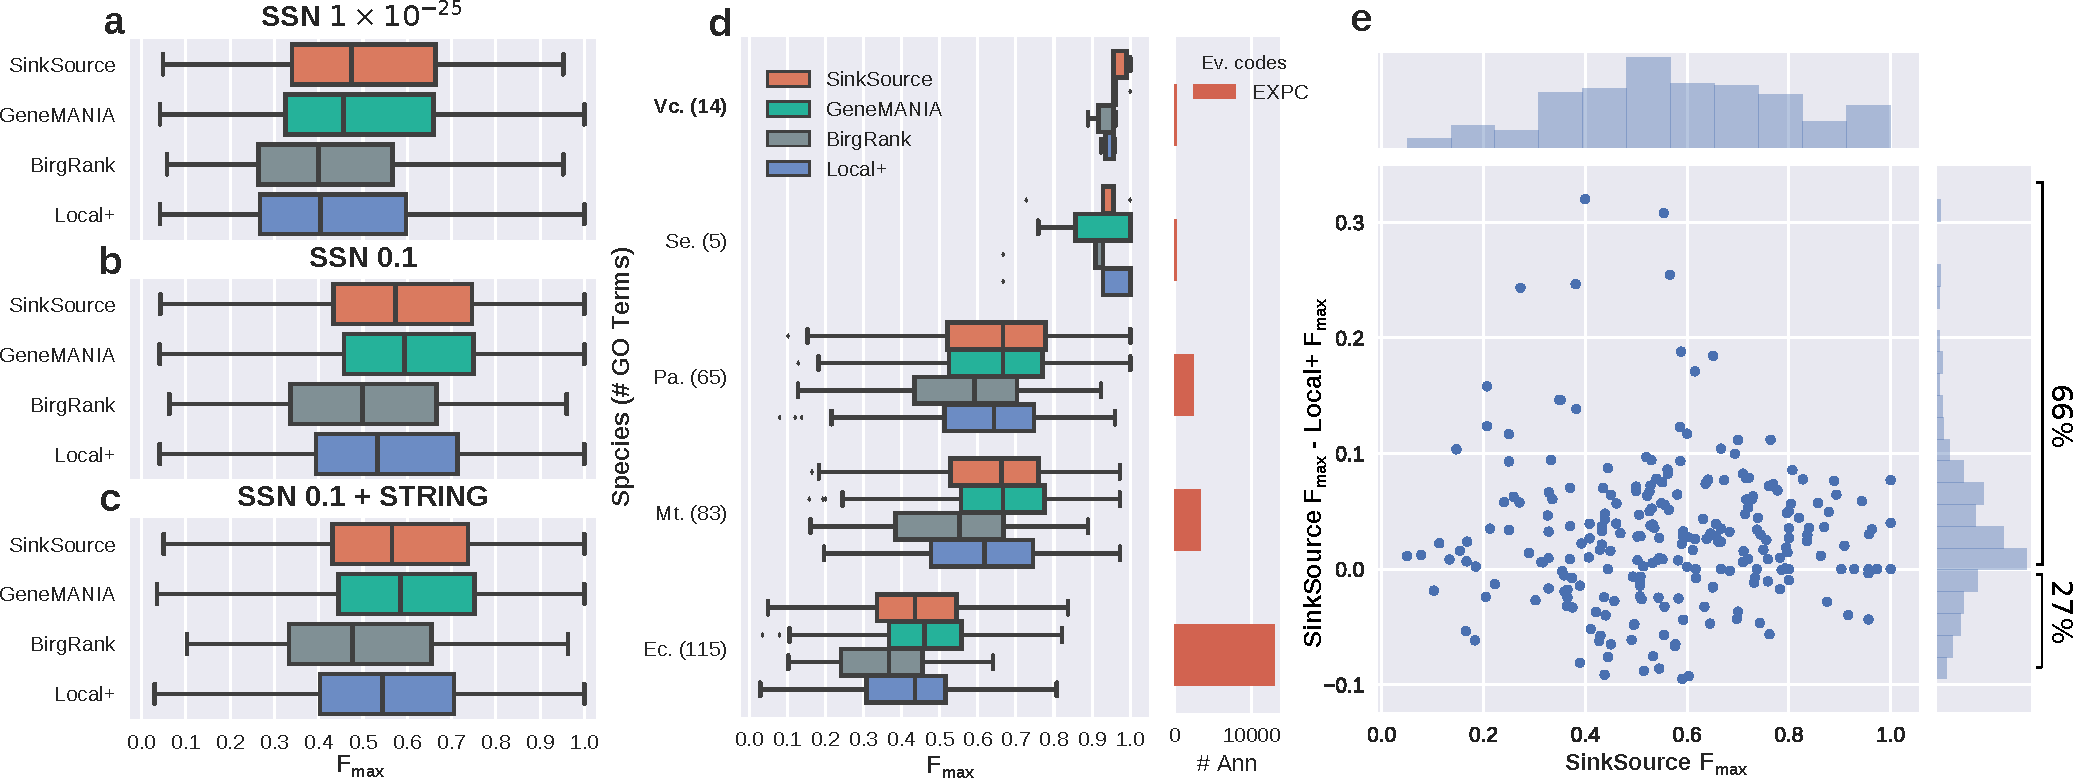
\includegraphics[width=\textwidth]{supp-figs/fig2-expc-compare-eval-fmax-sinksource-localplus-mf-a0_95.pdf}
    \caption{
      Comparison of \fmax results for \loso evaluation of four algorithms and three networks.
      (\textbf{a}) \SSN (\eval $\le$ \e{-25}),
      (\textbf{b}) \SSN (\eval $\le$ 0.1),
      (\textbf{c},\textbf{d},\textbf{e}) \SSN (\eval $\le$ 0.1) integrated with STRING,
      (\textbf{d}) \loso results for individual species, sorted in decreasing order of median \fmax. The number of MF GO terms with $\ge$ 10 annotations appears in parentheses next to each species name.  The species name is in bold if the difference between the distributions for \sinksource and \localplus was statistically significant (rank-sum Bonferroni-corrected \pval $< 0.05$). \protect The right-hand side shows the number of GO term-annotation pairs with experimental evidence codes for each species.
    %315 total BP GO terms have at least 10 annotations in the left-out species. 
    Species names are abbreviated as follows:
    \textit{Escherichia coli K-12} (Ec),
    \textit{Mycobacterium tuberculosis} (Mt),
    \textit{Neisseria gonorrhoeae} (Ng),
    \textit{Pseudomonas aeruginosa} (Pa),
    \textit{Salmonella enterica} (Se),
    \textit{Vibrio cholerae} (Vc),
    \textit{Yersinia pestis} (Yp).
    (\textbf{e}) Difference in \fmax between \sinksource and \localplus by the \fmax of \sinksource for each GO term. 
    %Comparison of using a \SSN with a cutoff of $1\times{}10^{-25}$ vs. a cutoff of $0.1$. The \fmax results for each individual species are combined and shown in a single box-plot for each algorithm.}
    }
    \label{fig:loso-results-exp-mf}
\end{figure}


\begin{figure} 
    \centering
    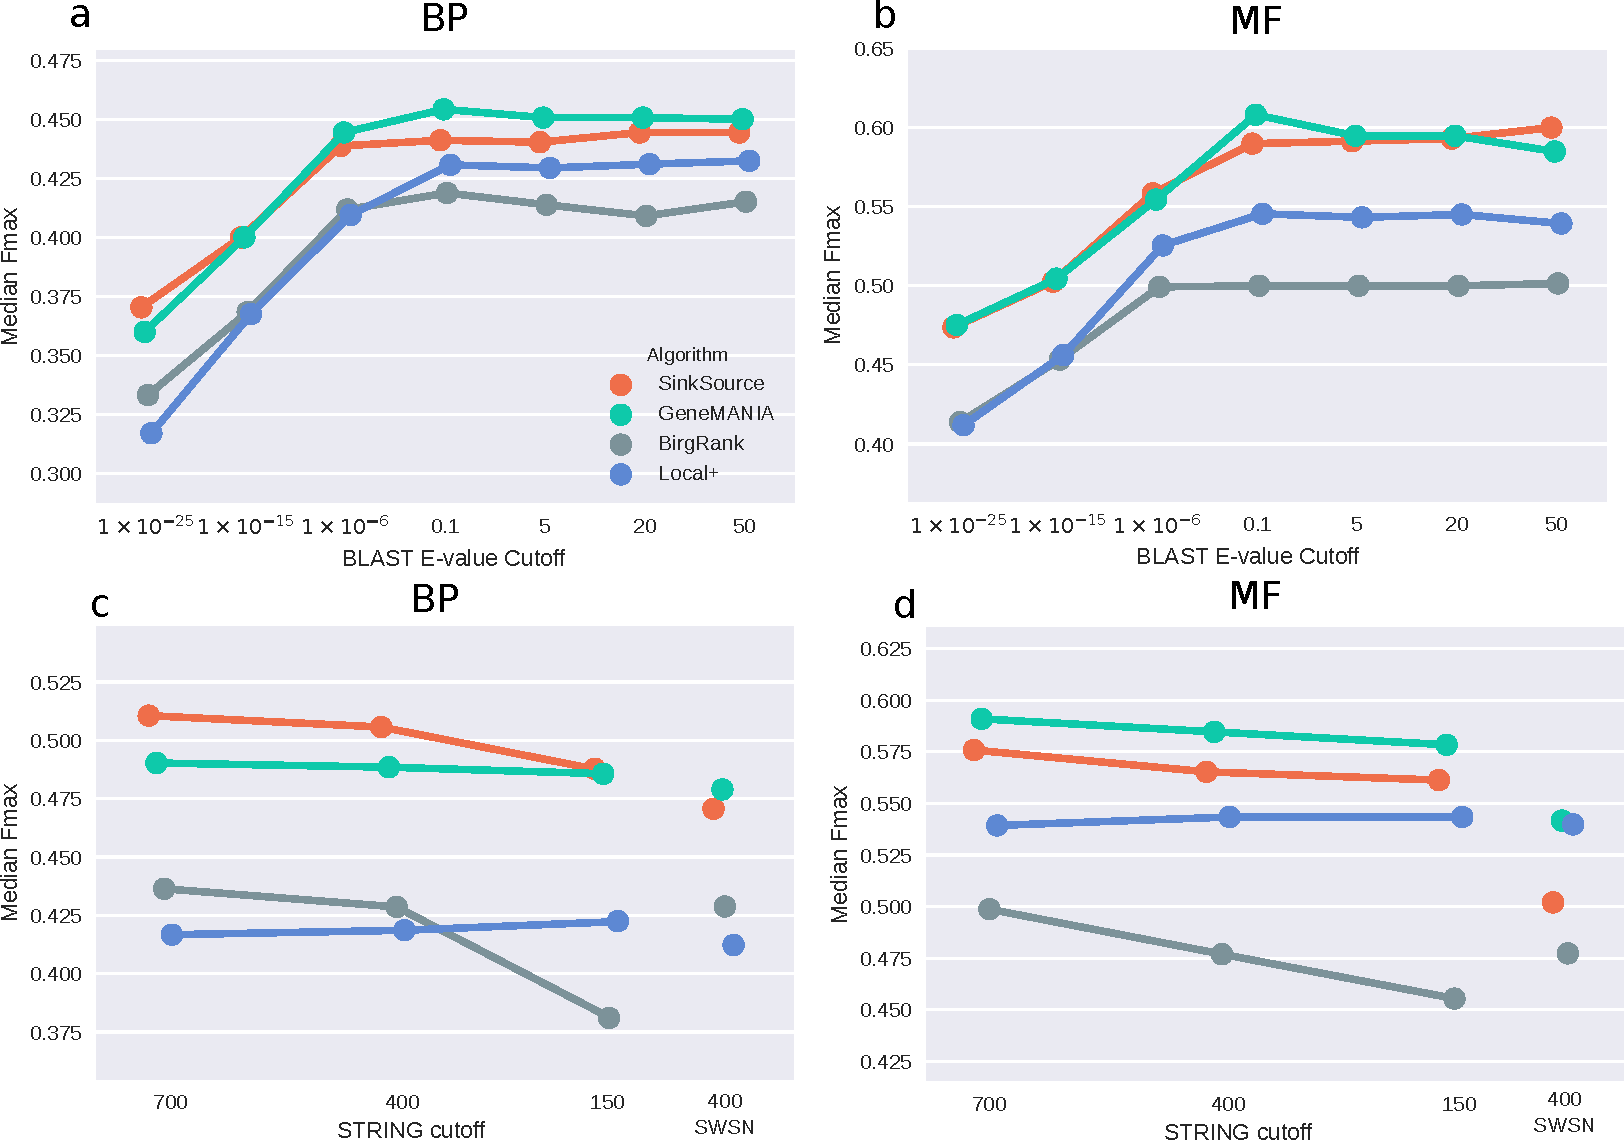
\includegraphics[width=\textwidth]{supp-figs/compare-eval-string-cutoffs-fmax-nobars.pdf}
    \caption{Comparison of \fmax results for \loso evaluation of EXPC annotations using various BLAST E-value cutoffs (\textbf{a}, \textbf{b}) and STRING cutoffs (\textbf{c}, \textbf{d}).
    For each algorithm and network, the plot shows the median \fmax as well as the 95\% confidence interval of the median using 1000 bootstrap samples.
    The last column of the \textbf{c} and \textbf{d} shows the results when using the SWSN method to weight the network with a STRING cutoff of 400.
    }
    \label{sfig:compare-eval-string-cutoffs}
\end{figure}


\begin{figure}
    \centering
    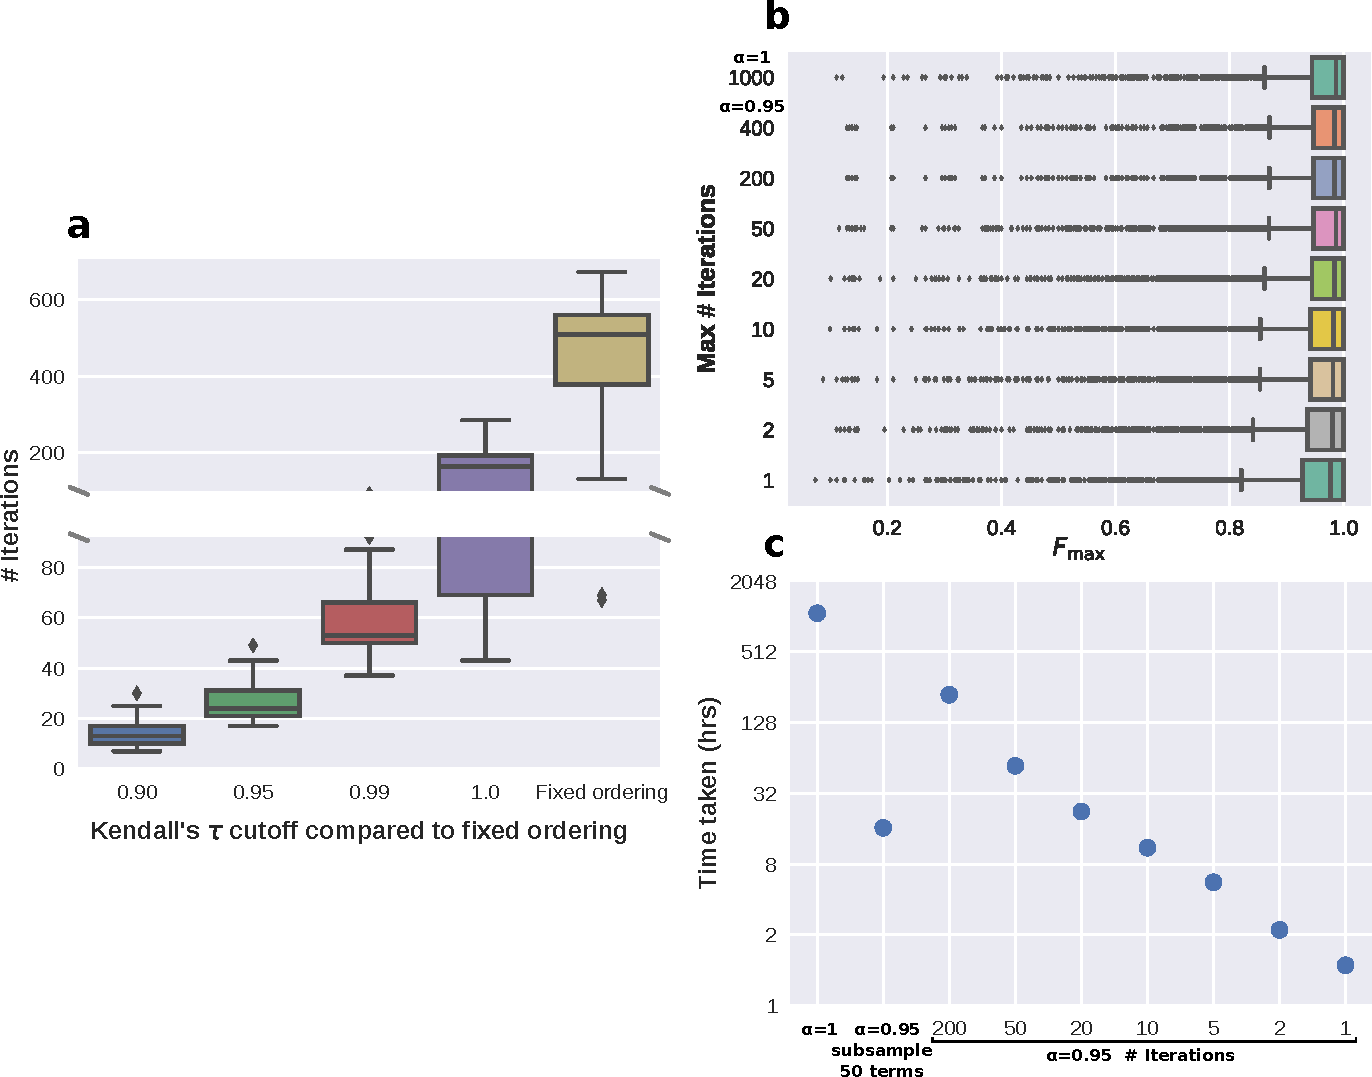
\includegraphics[width=\textwidth]{supp-figs/fig1-s200-expc-comp-rem-neg-iea-comp-bp-a0_95.pdf}
    \caption{Trade-off between accuracy and speed for SinkSource on the 200 bacterial species SSN (\eval $\leq$ 0.1) with 511 BP GO terms ($\geq 50$ annotations) for the LOSO evaluation using EXPC and COMP to make predictions, and COMP to evaluate in the left-out species.}
    \label{fig:my_label}
\end{figure}


\begin{figure}[H]
    \centering
    %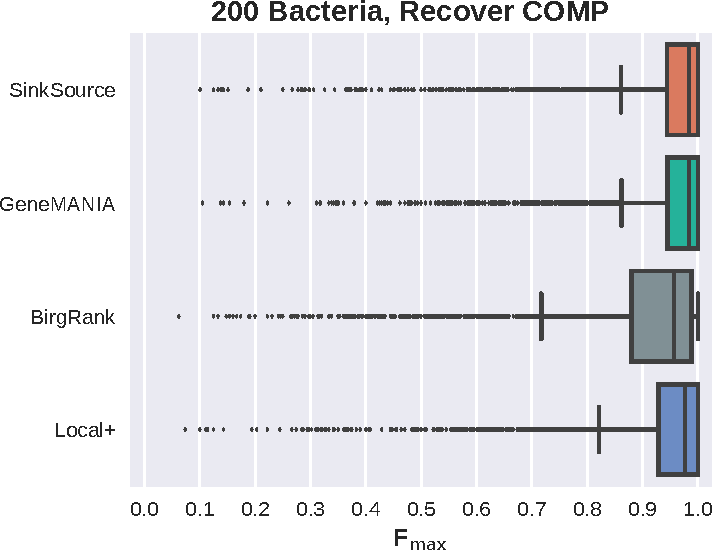
\includegraphics[width=\textwidth]{figs/s200-expc-comp-recover-comp-bp-4-use-neg-fmax-boxplot.pdf}
    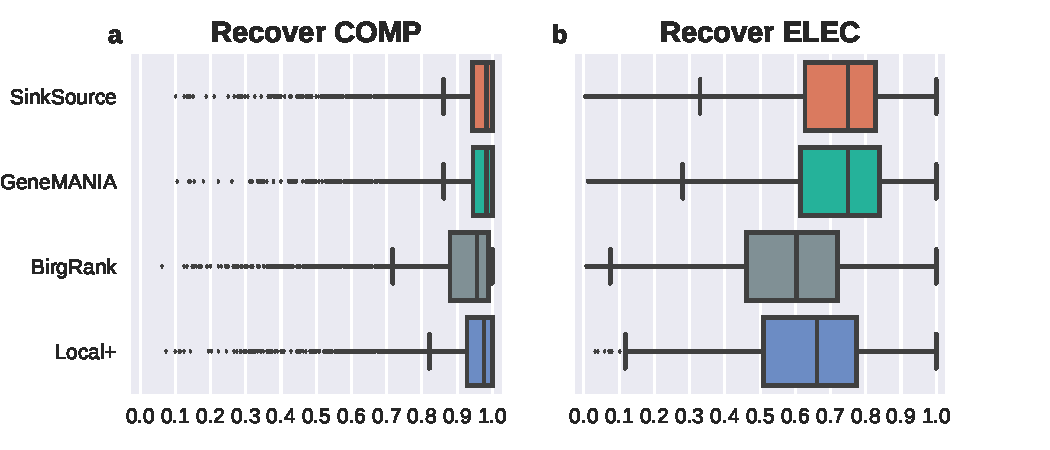
\includegraphics[width=\textwidth]{figs/s200-eval-comp-iea-fmax-boxplots-bp-0_95.pdf}
    \caption{
      Comparison of \fmax results of the \loso evaluation of different evidence codes using EXP and COMP annotations to make predictions for 200 bacterial species. 
      (\textbf{a}) Evaluation of recovery of COMP evidence codes of the left-out species.
      (\textbf{b}) Evaluation of recovery of ELEC evidence codes (IEA) of the left-out species.
    }
    \label{fig:s200-loso-results-expc-comp}
\end{figure}
